\section{CS 講義概要}
%
%%% GOAL
%
\subsection{講義の目標}
\begin{frame}
\frametitle{講義の目標}
  \begin{itemize}
\item 本講義では,このコンピュータサイエンスの基本をなす考え方を,課題を通して体得する
\item 物理現象をシミュレートしたり
\item 経済活動にともなう帳票類を管理したり
\item 機器を制御したり
\item コンピュータがいろいろな場面で利用されている
  \end{itemize}
\centering
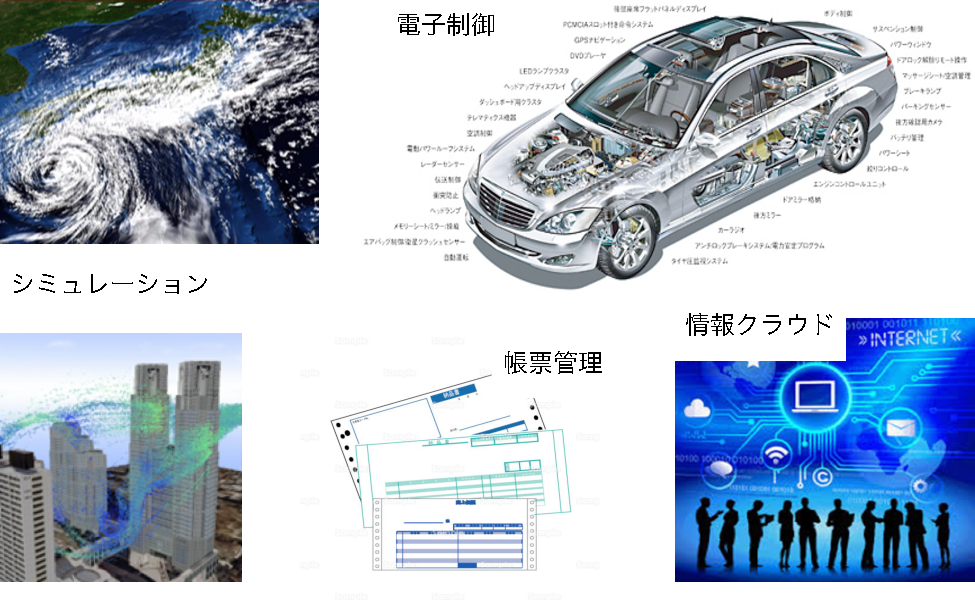
\includegraphics[scale=.35]{./Figure/elementaryCS-1st-FigComputer.pdf}
\end{frame}
\subsection{演習内容}
\begin{frame}
\frametitle{なぜコンピュータが利用できるのか}
  \begin{block}{コンピュータに載せるとは}
対象を\emph{計算}をもちいて表現し,コンピュータに処理させる
  \end{block}
  \begin{block}{目標}
    \begin{itemize}
\item CS 第一
      \begin{itemize}
\item 計算で表現するとは何か
\item コンピュータで処理するとは
      \end{itemize}
\item CS 第二 \href{https://wakita.github.io/classes/years/y22/cs2/course.html}{\beamerbutton{第二の講義概要}}
      \begin{itemize}
\item 計算の強力な道具 $\Rightarrow$ 再帰
\item 載せ方の上手下手があること $\Rightarrow$ アルゴリズムやデータ
      \end{itemize}
    \end{itemize}
  \end{block}
\end{frame}
\begin{frame}
\frametitle{演習内容}
  \begin{itemize}
\item 以下の演習を予定しています
  \end{itemize}
  \begin{block}{演習内容}
    \begin{itemize}
\item 演習課題 1: 四則演算でアニメーション
      \begin{itemize}
\item 計算の基本要素を知る
      \end{itemize}
\item 演習課題 2: 循環小数
      \begin{itemize}
\item 配列とは
      \end{itemize}
\item 演習課題 3: 暗号解読に挑戦
      \begin{itemize}
\item 文字列
\item サブルーチン
      \end{itemize}
\item 課題 S: 自然数から整数への拡張
    \end{itemize}
  \end{block}
\end{frame}
